\documentclass[11pt]{beamer}

% Add additional packages here, as needed

\usepackage{tikz}
\usepackage{textpos}
\usepackage{eso-pic}
\usepackage{ifthen}
\usepackage{intcalc}
\usepackage[serbian]{babel}
\usepackage[utf8]{inputenc}
\usepackage[T1]{fontenc}
\usepackage{listings}
\usepackage{anyfontsize}
\usepackage{bm}
\usepackage{amsfonts}
\usepackage{amsthm}
\usepackage{tikz}
\usepackage{mathtools}
\usepackage{clrscode3e}
\usepackage{mathrsfs}
\usepackage{pgfplots}

\usepackage{algorithm}
\usepackage[noend]{algpseudocode}
\usepackage{mathtools}

% za svg
\usepackage{graphicx}

\usepackage{hyperref}

\usetikzlibrary{decorations.pathreplacing}
\usetikzlibrary{shadows,positioning,calc}
\usetikzlibrary{arrows,decorations.pathmorphing,backgrounds,positioning,fit,petri}
\usetikzlibrary{shapes.geometric, automata, chains}
\usetikzlibrary{matrix, positioning}
\tikzstyle{inputNode}=[draw,circle,minimum size=10pt,inner sep=0pt]
\tikzstyle{stateTransition}=[-stealth, thick]
\renewcommand{\ttdefault}{cmtt}

\useoutertheme[subsection=false,footline=authortitle]{miniframes}

\usecolortheme{orchid}

\setbeamercolor{navigation symbols dimmed}{fg=white}
\setbeamercolor{navigation symbols}{fg=white}

\definecolor{uorange}{HTML}{e60b42}
\definecolor{canaub}{HTML}{F09A00}
\definecolor{coolgrey}{HTML}{111111}
\definecolor{lgry}{HTML}{cccccc}

\setbeamercolor{title}{fg=white, bg=uorange}
\setbeamercolor{frametitle}{fg=white, bg=uorange}
\setbeamercolor{section in head/foot}{fg=lgry, bg=coolgrey}
\setbeamercolor{subsection in head/foot}{fg=coolgrey, bg=canaub}
\setbeamercolor{background canvas}{bg=white}
\setbeamercolor{itemize item}{fg=coolgrey}
\setbeamercolor{itemize subitem}{fg=coolgrey}
\setbeamercolor{normal text}{fg=coolgrey}
\setbeamercolor{block title}{fg=white,bg=uorange}

\newcommand\Proba{\mathbb{P}}
\newtheorem*{mytheorem}{Дефиниција}
\newtheorem*{teorema}{Теорема}
\newtheorem*{mycorollary}{Posledica}
\DeclareMathOperator{\argmax}{argmax} % no space, limits on side in displays

\frenchspacing

\addtobeamertemplate{title page}{}{%
\begin{textblock*}{\paperwidth}(0.02cm,-9.185cm)
\begin{tikzpicture}
	\fill[rectangle, fill=white, opacity=0.5] (-1, 0) rectangle (9.76, 0.04);
\end{tikzpicture}
\end{textblock*}}

\addtobeamertemplate{frametitle}{}{%
\begin{textblock*}{100mm}(\textwidth,-0.845cm)
\end{textblock*}}

\addtobeamertemplate{frametitle}{}{%
\begin{textblock*}{\paperwidth}(-0.98cm,-0.94cm)
\begin{tikzpicture}
	\fill[rectangle, fill=white, opacity=0.5] (-1, 0) rectangle (11.76, 0.04);
\end{tikzpicture}
\end{textblock*}}

\newcommand{\glidera}[1]{\tikz{
		\draw[fill=uorange,draw=none] (0, 0) rectangle(#1, #1);%%
		\draw[fill=uorange,draw=none] (-2*#1, #1) rectangle(-#1, 2*#1);
		\draw[fill=uorange,draw=none] (-#1, #1) rectangle(0, 2*#1);
		\draw[fill=uorange,draw=none] (0, #1) rectangle(#1, 2*#1);
		\draw[fill=uorange,draw=none] (#1, #1) rectangle(2*#1, 2*#1);%%
		\draw[fill=uorange,draw=none] (-3*#1, 2*#1) rectangle(-2*#1, 3*#1);
		\draw[fill=uorange,draw=none] (-#1, 2*#1) rectangle(0, 3*#1);
		\draw[fill=uorange,draw=none] (#1, 2*#1) rectangle(2*#1, 3*#1);
		\draw[fill=uorange,draw=none] (2*#1, 2*#1) rectangle(3*#1, 3*#1);%%
		\draw[fill=uorange,draw=none] (-4*#1, 3*#1) rectangle(-3*#1, 4*#1);
		\draw[fill=uorange,draw=none] (-#1, 3*#1) rectangle(0, 4*#1);
		\draw[fill=uorange,draw=none] (#1, 3*#1) rectangle(2*#1, 4*#1);
		\draw[fill=uorange,draw=none] (2*#1, 3*#1) rectangle(3*#1, 4*#1);
		\draw[fill=uorange,draw=none] (3*#1, 3*#1) rectangle(4*#1, 4*#1);%%
		\draw[fill=uorange,draw=none] (-3*#1, 4*#1) rectangle(-2*#1, 5*#1);
		\draw[fill=uorange,draw=none] (-#1, 4*#1) rectangle(0, 5*#1);
		\draw[fill=uorange,draw=none] (#1, 4*#1) rectangle(2*#1, 5*#1);
		\draw[fill=uorange,draw=none] (2*#1, 4*#1) rectangle(3*#1, 5*#1);%%
		\draw[fill=uorange,draw=none] (-2*#1, 5*#1) rectangle(-#1, 6*#1);
		\draw[fill=uorange,draw=none] (-#1, 5*#1) rectangle(0, 6*#1);
		\draw[fill=uorange,draw=none] (0, 5*#1) rectangle(#1, 6*#1);
		\draw[fill=uorange,draw=none] (#1, 5*#1) rectangle(2*#1, 6*#1);%%
		\draw[fill=uorange,draw=none] (0, 6*#1) rectangle(#1, 7*#1);%%
	}}
	
\newcommand{\gliderb}[1]{\tikz{
		\draw[fill=uorange,draw=none] (0, 0) rectangle(#1, #1);
		\draw[fill=uorange,draw=none] (#1, 0) rectangle(2*#1, #1);%%
		\draw[fill=uorange,draw=none] (-2*#1, #1) rectangle(-#1, 2*#1);
		\draw[fill=uorange,draw=none] (2*#1, #1) rectangle(3*#1, 2*#1);%%
		\draw[fill=uorange,draw=none] (-3*#1, 2*#1) rectangle(-2*#1, 3*#1);
		\draw[fill=uorange,draw=none] (3*#1, 2*#1) rectangle(4*#1, 3*#1);%%
		\draw[fill=uorange,draw=none] (-4*#1, 3*#1) rectangle(-3*#1, 4*#1);
		\draw[fill=uorange,draw=none] (-3*#1, 3*#1) rectangle(-2*#1, 4*#1);
		\draw[fill=uorange,draw=none] (-#1, 3*#1) rectangle(0, 4*#1);
		\draw[fill=uorange,draw=none] (3*#1, 3*#1) rectangle(4*#1, 4*#1);%%
		\draw[fill=uorange,draw=none] (-3*#1, 4*#1) rectangle(-2*#1, 5*#1);
		\draw[fill=uorange,draw=none] (3*#1, 4*#1) rectangle(4*#1, 5*#1);%%
		\draw[fill=uorange,draw=none] (-2*#1, 5*#1) rectangle(-#1, 6*#1);
		\draw[fill=uorange,draw=none] (2*#1, 5*#1) rectangle(3*#1, 6*#1);%%
		\draw[fill=uorange,draw=none] (0, 6*#1) rectangle(#1, 7*#1);
		\draw[fill=uorange,draw=none] (#1, 6*#1) rectangle(2*#1, 7*#1);%%
	}}
	
\newcommand{\gliderc}[1]{\tikz{
		\draw[fill=uorange,draw=none] (0, 0) rectangle(#1, #1);%%
		\draw[fill=uorange,draw=none] (0, #1) rectangle(#1, 2*#1);
		\draw[fill=uorange,draw=none] (#1, #1) rectangle(2*#1, 2*#1);%%
		\draw[fill=uorange,draw=none] (-5*#1, 2*#1) rectangle(-4*#1, 3*#1);
		\draw[fill=uorange,draw=none] (-4*#1, 2*#1) rectangle(-3*#1, 3*#1);
		\draw[fill=uorange,draw=none] (#1, 2*#1) rectangle(2*#1, 3*#1);
		\draw[fill=uorange,draw=none] (2*#1, 2*#1) rectangle(3*#1, 3*#1);%%
		\draw[fill=uorange,draw=none] (-5*#1, 3*#1) rectangle(-4*#1, 4*#1);
		\draw[fill=uorange,draw=none] (-4*#1, 3*#1) rectangle(-3*#1, 4*#1);
		\draw[fill=uorange,draw=none] (#1, 3*#1) rectangle(2*#1, 4*#1);
		\draw[fill=uorange,draw=none] (2*#1, 3*#1) rectangle(3*#1, 4*#1);
		\draw[fill=uorange,draw=none] (3*#1, 3*#1) rectangle(4*#1, 4*#1);%%
		\draw[fill=uorange,draw=none] (-5*#1, 4*#1) rectangle(-4*#1, 5*#1);
		\draw[fill=uorange,draw=none] (-4*#1, 4*#1) rectangle(-3*#1, 5*#1);
		\draw[fill=uorange,draw=none] (#1, 4*#1) rectangle(2*#1, 5*#1);
		\draw[fill=uorange,draw=none] (2*#1, 4*#1) rectangle(3*#1, 5*#1);%%
		\draw[fill=uorange,draw=none] (0, 5*#1) rectangle(#1, 6*#1);
		\draw[fill=uorange,draw=none] (#1, 5*#1) rectangle(2*#1, 6*#1);%%
		\draw[fill=uorange,draw=none] (0, 6*#1) rectangle(#1, 7*#1);%%
	}}
	
\newcommand{\gliderd}[1]{\tikz{
		\draw[fill=uorange,draw=none] (0, 0) rectangle(#1, #1);
		\draw[fill=uorange,draw=none] (#1, 0) rectangle(2*#1, #1);%%
		\draw[fill=uorange,draw=none] (0, #1) rectangle(#1, 2*#1);
		\draw[fill=uorange,draw=none] (2*#1, #1) rectangle(3*#1, 2*#1);%%
		\draw[fill=uorange,draw=none] (-5*#1, 2*#1) rectangle(-4*#1, 3*#1);
		\draw[fill=uorange,draw=none] (-4*#1, 2*#1) rectangle(-3*#1, 3*#1);
		\draw[fill=uorange,draw=none] (3*#1, 2*#1) rectangle(4*#1, 3*#1);%%
		\draw[fill=uorange,draw=none] (-6*#1, 3*#1) rectangle(-5*#1, 4*#1);
		\draw[fill=uorange,draw=none] (-3*#1, 3*#1) rectangle(-2*#1, 4*#1);
		\draw[fill=uorange,draw=none] (0, 3*#1) rectangle(#1, 4*#1);
		\draw[fill=uorange,draw=none] (3*#1, 3*#1) rectangle(4*#1, 4*#1);%%
		\draw[fill=uorange,draw=none] (-5*#1, 4*#1) rectangle(-4*#1, 5*#1);
		\draw[fill=uorange,draw=none] (-4*#1, 4*#1) rectangle(-3*#1, 5*#1);
		\draw[fill=uorange,draw=none] (3*#1, 4*#1) rectangle(4*#1, 5*#1);%%
		\draw[fill=uorange,draw=none] (0, 5*#1) rectangle(#1, 6*#1);
		\draw[fill=uorange,draw=none] (2*#1, 5*#1) rectangle(3*#1, 6*#1);%%
		\draw[fill=uorange,draw=none] (0, 6*#1) rectangle(#1, 7*#1);
		\draw[fill=uorange,draw=none] (#1, 6*#1) rectangle(2*#1, 7*#1);%%
	}}
	
\newcommand{\glidere}[1]{\tikz{
		\draw[fill=uorange,draw=none] (0, 0) rectangle(#1, #1);
		\draw[fill=uorange,draw=none] (#1, 0) rectangle(2*#1, #1);%%
		\draw[fill=uorange,draw=none] (0, #1) rectangle(#1, 2*#1);
		\draw[fill=uorange,draw=none] (2*#1, #1) rectangle(3*#1, 2*#1);%%
		\draw[fill=uorange,draw=none] (-5*#1, 2*#1) rectangle(-4*#1, 3*#1);
		\draw[fill=uorange,draw=none] (-4*#1, 2*#1) rectangle(-3*#1, 3*#1);
		\draw[fill=uorange,draw=none] (#1, 2*#1) rectangle(2*#1, 3*#1);
		\draw[fill=uorange,draw=none] (2*#1, 2*#1) rectangle(3*#1, 3*#1);
		\draw[fill=uorange,draw=none] (3*#1, 2*#1) rectangle(4*#1, 3*#1);%%
		\draw[fill=uorange,draw=none] (-6*#1, 3*#1) rectangle(-5*#1, 4*#1);
		\draw[fill=uorange,draw=none] (-3*#1, 3*#1) rectangle(-2*#1, 4*#1);
		\draw[fill=uorange,draw=none] (2*#1, 3*#1) rectangle(3*#1, 4*#1);
		\draw[fill=uorange,draw=none] (3*#1, 3*#1) rectangle(4*#1, 4*#1);
		\draw[fill=uorange,draw=none] (4*#1, 3*#1) rectangle(5*#1, 4*#1);%%
		\draw[fill=uorange,draw=none] (-5*#1, 4*#1) rectangle(-4*#1, 5*#1);
		\draw[fill=uorange,draw=none] (-4*#1, 4*#1) rectangle(-3*#1, 5*#1);
		\draw[fill=uorange,draw=none] (#1, 4*#1) rectangle(2*#1, 5*#1);
		\draw[fill=uorange,draw=none] (2*#1, 4*#1) rectangle(3*#1, 5*#1);
		\draw[fill=uorange,draw=none] (3*#1, 4*#1) rectangle(4*#1, 5*#1);%%
		\draw[fill=uorange,draw=none] (0, 5*#1) rectangle(#1, 6*#1);
		\draw[fill=uorange,draw=none] (2*#1, 5*#1) rectangle(3*#1, 6*#1);%%
		\draw[fill=uorange,draw=none] (0, 6*#1) rectangle(#1, 7*#1);
		\draw[fill=uorange,draw=none] (#1, 6*#1) rectangle(2*#1, 7*#1);%%
	}}
	
\newcommand{\gla}[1]{\tikz{
		\draw[fill=uorange,draw=none] (0, 0) rectangle(#1, #1);
		\draw[fill=uorange,draw=none] (#1, 0) rectangle(2*#1, #1);
		\draw[fill=uorange,draw=none] (2*#1, 0) rectangle(3*#1, #1);%%
		\draw[fill=uorange,draw=none] (2*#1, #1) rectangle(3*#1, 2*#1);%%
		\draw[fill=uorange,draw=none] (#1, 2*#1) rectangle(2*#1, 3*#1);%%
	}}
\newcommand{\glb}[1]{\tikz{
		\draw[fill=uorange,draw=none] (0, 0) rectangle(#1, #1);%%
		\draw[fill=uorange,draw=none] (0, #1) rectangle(#1, 2*#1);
		\draw[fill=uorange,draw=none] (#1, #1) rectangle(2*#1, 2*#1);%%
		\draw[fill=uorange,draw=none] (-#1, 2*#1) rectangle(0, 3*#1);
		\draw[fill=uorange,draw=none] (#1, 2*#1) rectangle(2*#1, 3*#1);%%
	}}
\newcommand{\glc}[1]{\tikz{
		\draw[fill=uorange,draw=none] (0, 0) rectangle(#1, #1);
		\draw[fill=uorange,draw=none] (#1, 0) rectangle(2*#1, #1);%%
		\draw[fill=uorange,draw=none] (-#1, #1) rectangle(0, 2*#1);
		\draw[fill=uorange,draw=none] (#1, #1) rectangle(2*#1, 2*#1);%%
		\draw[fill=uorange,draw=none] (#1, 2*#1) rectangle(2*#1, 3*#1);%%
	}}
\newcommand{\gld}[1]{\tikz{
		\draw[fill=uorange,draw=none] (0, 0) rectangle(#1, #1);
		\draw[fill=uorange,draw=none] (#1, 0) rectangle(2*#1, #1);%%
		\draw[fill=uorange,draw=none] (#1, #1) rectangle(2*#1, 2*#1);
		\draw[fill=uorange,draw=none] (2*#1, #1) rectangle(3*#1, 2*#1);%%
		\draw[fill=uorange,draw=none] (0, 2*#1) rectangle(#1, 3*#1);%%
	}}

\newcommand{\gun}[1]{%
	\ifthenelse{\equal{\intcalcMod{\value{#1}}{5}}{1}}{%
		\glidera{0.035}%
	}{%
		\ifthenelse{\equal{\intcalcMod{\value{#1}}{5}}{2}}{
			\gliderb{0.035}%
		}{%
			\ifthenelse{\equal{\intcalcMod{\value{#1}}{5}}{3}}{
				\gliderc{0.035}%
			}{%
				\ifthenelse{\equal{\intcalcMod{\value{#1}}{5}}{4}}{
					\gliderd{0.035}%
				}{%
					\glidere{0.035}%
				}%
			}%
		}%
	}%
}

\newcommand{\gli}[1]{%
	\ifthenelse{\equal{\intcalcMod{\value{#1}}{4}}{1}}{%
		\gla{0.09}
	}{%
		\ifthenelse{\equal{\intcalcMod{\value{#1}}{4}}{2}}{
			\glb{0.09}
		}{%
			\ifthenelse{\equal{\intcalcMod{\value{#1}}{4}}{3}}{
				\glc{0.09}
			}{%
				\gld{0.09}
			}%
		}{}%
	}{}%
}
	
\setbeamertemplate{enumerate item}{\gli{enumi}}
\setbeamertemplate{enumerate subitem}{\gun{enumii}}

%%%%%%%%%%%%%%%%%%%%%%%%%%%%%%%%%%%%%%%%%%%%%%%%%%
% Essential data about the presentation goes here

\title{PageRank algoritam na Wikipediji}
\author[\textcolor{lgry}{Vuk Vuković 0119/17\\ Filip Vesović 0018/17}]{Vuk Vuković 0119/17\\ Filip Vesović 0018/17}
\date{Jun 2019.}
\institute{\textcolor{uorange}{\scshape Verovatnoća i statistika (13S082VS)}\\
Elektrotehnički fakultet,\\
Univerzitet u Beogradu}

%%%%%%%%%%%%%%%%%%%%%%%%%%%%%%%%%%%%%%%%%%%%%%%%%%

\begin{document}

{
    \setbeamertemplate{headline}{} 
    \begin{frame}
        \titlepage

    \end{frame}
}

\section{Uvod}
\subsection{Uvod}

\begin{frame}
    \frametitle{Uvod}
  		\begin{center}
        \begin{enumerate}
                \item Prvi internet pretraživači
                \item Google - više stotina milijardi indeksiranih stranica
                \item Koje stranice prikazati korisniku za zadatu pretragu?
                \item Po kom redosledu sortirati stranice ukoliko je dostupno više rezultata?
            \end{enumerate}
            
\includegraphics[width=0.4\columnwidth]{pretrazivaci.png}
        \end{center}
\end{frame}

\begin{frame}
    \frametitle{PageRank algoritam}
  		\begin{center}
            \begin{enumerate}
                \item Larry Page i Sergey Brin 
                \item Studenti doktorskih studija, Univerzitet Stanford
                \item 1996. razvijaju PageRank algoritam kao deo istraživačkog projekta o internet servisu za pretragu
                \item Glavna ideja: rangiranje informacija na internetu po kredibilitetu (bitnosti stranica na kojima se one nalaze)
                \item Bitnost jedne stranice zavisi kako od stranica koje nju linkuju, tako i bitnosti tih stranica
                \item Nakon nekoliko godina osnivaju Google
            \end{enumerate}
        \end{center}
\end{frame}
\begin{frame}
    \frametitle{PageRank algoritam danas}
  		\begin{center}
            \begin{enumerate}
                \item Koristi se kao jedan od kriterijuma na osnovu kojih se rangiraju rezultati pretrage
                \item Google ovaj algoritam izvršava neprestano na velikom broju servera
                \item Primena algoritma na manji skup podataka
                \item Engleska verzija slobodne enciklopedije Wikipedia dosutpna za preuzimanje
            \end{enumerate}
        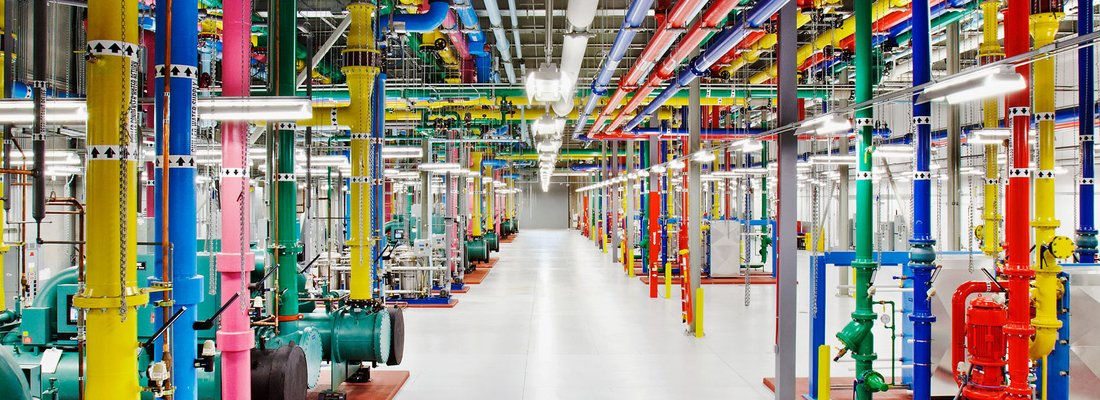
\includegraphics[width=0.8\columnwidth]{datacenter.jpg}
        \end{center}
\end{frame}

\section{Teorijski uvod}
\subsection{Teorijski uvod}
\begin{frame}
    \frametitle{Slučajni procesi}
  		\begin{center}
        \begin{enumerate}
                \item Slučajni proces je familija slučajnih promenjivih $\{X_t\}_{t \in T}$
               \item Ako je skup $T$ diskretan tada se radi o slučajnom procesu sa diskretnim vremenom
                \item Skup svih mogućih vrednosti slučajnih promenljivih $X_t$ za $t \in T$ zove se skup stanja procesa $X_t$ \textit{(Merkle 2016)}
            \end{enumerate}
        \end{center}
\end{frame}

\begin{frame}
    \frametitle{Markovski lanac}
  		\begin{center}
        \begin{enumerate}
                \item Markovski lanac predstavlja slučajni proces sa diskretnim vremenom i konačnim skupom stanja
                \item U svakom Markovskom lancu važi da verovatnoća prelaska iz stanja $X_k$ u stanje $X_{k+1}$ ne zavisi od stanja u kojima je sistem bio u prethodnim trenucima, već isključivo od trenutnog stanja $X_k$ (osobina Markova)
            \end{enumerate}
            \begin{equation*}
\begin{aligned}
P(X_{k+1} = x | X_{1} = x_{1}, X_{2} = x_{2}, ...,  X_{k} = x_{k}) =\\ P(X_{k+1} = x| X_{k} = x_{k})
\end{aligned}
\end{equation*}
        \end{center}
\end{frame}

\begin{frame}
    \frametitle{Primer (Markovski lanac)}
  		\begin{center}
\begin{figure}[h]
\centering{
\resizebox{90mm}{!}{\input{markov_chain.pdf_tex}}
}
\end{figure}
        \end{center}
\end{frame}

\begin{frame}
    \frametitle{Iterativni metodi}
  		\begin{center}
            \begin{enumerate}
                \item Metodi koji na osnovu početne pretpostavke i zadatog algoritma, iterativno menjaju rešenje
                \item Konvergencija (sekvenca iteracija konvergira za zadate početne uslove)
                \item Striktnu matematička pozadina nije obrađena s obzirom da se radi o inženjerskom algoritmu pre svega zasnovanog na intuitivnim pretpostavkama
            \end{enumerate}
            \leavevmode \\
        \resizebox{60mm}{!}{$X_0, X_1, X_2, ..., X_k, ... X_{\infty}$}
        \end{center}
\end{frame}

\begin{frame}
    \frametitle{PageRank algoritam}
  		\begin{center}
            \begin{enumerate}
                \item Određivanje verovatnoća da će se nasumični korisnik pronaći na određenoj stranici posle (beskonačno) mnogo koraka
                \item Inicijalno, svaka stranica ima jednaku verovatnoću nalaska korisnika
                \item Iterativnim postupkom na osnovu raspodele verovatnoća u trenutku $t = k$ određuje se raspodela verovatnoća u narednom trenutku $t = k+1$
                \item Nije moguće odrediti krajnje rešenje konvergencije ($t = \infty$)
                \item Prekid rada kada razlika između dve uzastopne raspodele padne ispod unapred definisane vrednosti
            \end{enumerate}
        \end{center}
\end{frame}

\begin{frame}
    \frametitle{PageRank algoritam}
  		    Model Markovljevih lanaca koji PageRank koristi je sledeći \textit{(Page et al., 1999)}:
            \begin{enumerate}
                \item Svaka stranica predstavlja jedno od mogućih stanja
                \item Sa svake stranice moguće je preći na bilo koju drugu stranicu sa verovatnoćom $\delta$
                \item Preostala verovatnoća $1 - \delta$ je uniformno raspodeljenja za prelazak na linkove te stranice ($\frac{1-\delta}{L}$, gde $L$ predstavlja ukupan broj linkova na stranici)
            \end{enumerate}
\end{frame}

\begin{frame}
    \frametitle{Faktor odbacivanja}
  		\begin{center}
            \begin{enumerate}
                \item Parameter $\delta$ se još naziva i stepenom odbacivanja (engl. \textit{Damping factor)}
                \item Postojanje verovatnoće da korisnik umesto klika na neki od linkova na stranici pređe na drugu stranicu unošenjem adrese stranice direktno (ili pretragom)
                \item Neophodan za ispravan rad algoritma
                \item Stranice bez izlaznih linkova bi imale najveći PageRank (korisnici ih ne mogu napustiti)
            \end{enumerate}
            \leavevmode \\
            
\includegraphics[width=0.4\columnwidth]{url.jpg}
        \end{center}
\end{frame}

\begin{frame}
    \frametitle{Mera bitnosti (relevantnosti)}
    Smisao PageRank-a kao mere bitnosti stranica na internetu:
  		\begin{center}
            \begin{enumerate}
                \item Stranice koje imaju više linkova ka njima teže da imaju veći PageRank (više stranica se oslanja na nju, smtraju je bitnom i verodostojnom)
                \item Stranice koje imaju veći PageRank doprinose značajnije PageRank-u stranica koje linkuju nego one sa manjim (pokazatelj verodostojnosti jeste ukoliko se neka verodostojna stranica oslanja na nju)
            \end{enumerate}
        \end{center}
\end{frame}

\begin{frame}
    \frametitle{PageRank primer}
  		\begin{center}
\begin{figure}[h]
\centering{
\resizebox{100mm}{!}{\input{primer_kratko.pdf_tex}}
}
\end{figure}
        \end{center}
\end{frame}

\begin{frame}
    \frametitle{PageRank primer}
  		\begin{center}
\begin{table}[]
\centering
\begin{tabular}{|l|l|l|l|l|l|l|}
\hline
    & ETF & RTI & Matematika  & SIS & Elektronika  \\ \hline
0   & 0.2000  & 0.2000 &  0.2000  & 0.2000  &  0.2000   \\ \hline
1   & 0.1667  & 0.3500 &  0.3167  & 0.1167  &  0.0500   \\ \hline
2   & 0.1917  & 0.4167 &  0.2917  & 0.0583  &  0.0417   \\ \hline
3   & 0.2222  & 0.3688 &  0.2993  & 0.0618  &  0.0479   \\ \hline
4   & 0.2003  & 0.3858 &  0.2868  & 0.0715  &  0.0554  \\ \hline
$\infty$   & 0.2069  & 0.3793 &  0.2931  & 0.0690  &  0.0517 \\ \hline
\end{tabular}
\end{table}
    \begin{enumerate}
        \item Za koju stranicu bismo intuitivno rekli da će imati najveći PageRank?
        \item Da li se to poklapa sa rezultatima?
    \end{enumerate}
        \end{center}
\end{frame}

\begin{frame}
\frametitle{Algoritam}
\begin{center}
   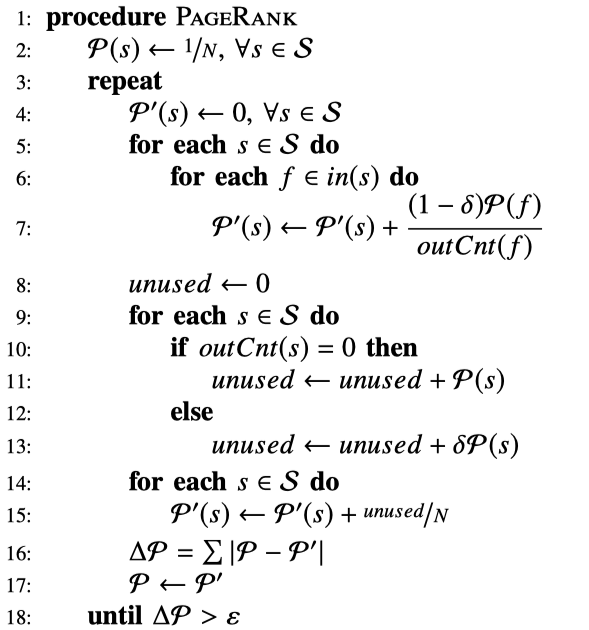
\includegraphics[width=0.6\columnwidth]{algoritam.png}
\end{center}
\end{frame}

\section{Implementacija}
\subsection{Implementacija}

\begin{frame}
    \frametitle{Wikipedia}
  		\begin{center}
        \begin{enumerate}
            \item Dozvoljava preuzimanje čitave engleske verzije (5,5 miliona članaka)
            \item XML datoteka od preko 70GB 
            \item Svaki članak se sastoji od naslova, određenih tehničkih podataka i sadržaja
            \item Interni i eksterni linkovi (odbačeni eksterni, šablonski i kategorijski)
        \end{enumerate}
        \end{center}
        \leavevmode \\
        \begin{flushright}
            
\includegraphics[width=0.25\columnwidth]{wiki.png}
        \end{flushright}
\end{frame}

\begin{frame}
    \frametitle{Obrada podataka}
\begin{center}
    \begin{enumerate}
    \item Program za obradu podataka napisan u C++
    \item Svaki članak opisan je na sledeći način:
        \begin{enumerate}
        \item Naziv članka
        \item Automatski dodeljen identifikator
        \item Niz identifikatora članaka koje posmatrani članak linkuje
        \end{enumerate}
        \item S obzirom na količinu podataka, trajanje obrade podataka i izdvajanja potrebnog sadržaja je oko 2.5 časa
        \item Obradom 72 GB dobijeno je oko 2.6 GB podataka nad kojima je rađen PageRank algoritam
    \end{enumerate}

        \end{center}
\end{frame}

\begin{frame}
    \frametitle{Primena PageRank algoritma}
  		\begin{center}
        \begin{enumerate}
        \item Kod samog algoritma takođe je napisan u C++
        \item Faktor odbacivanja koji je korišćen je $\delta = 0.1$
        \item 150 iteracija
        \item Krajna greška od $7 \cdot 10^{-12}$ za šta je bilo potrebno oko 15 minuta
        \item Vreme potrebno za računanje jedne iteracije je oko 6,5 sekundi
        \item Krajnji rezultat predstavlja sortirana lista imena članaka i njihovih verovatnoća od oko 500 MB
        \end{enumerate}
        \end{center}
\end{frame}

\section{Rezultati}
\subsection{Rezultati}

\begin{frame}
    \frametitle{Prvih 20 stranica}
  		\begin{center}
  		\begin{table}[]
\begin{tabular}{|l|l|l|l|}
\hline
1.  & United States                                  & 11. & List Of Sovereign States \\ \hline
2.  & World War II                                   & 12. & Association Football     \\ \hline
3.  & United Kingdom                                 & 13. & Italy                    \\ \hline
4.  & France                                         & 14. & Canada                   \\ \hline
5.  & Race And Ethnicity In The US & 15. & Australia                \\ \hline
6.  & Germany                                        & 16. & The New York Times       \\ \hline
7.  & India                                          & 17. & London                   \\ \hline
8.  & New York City                                  & 18. & English Language         \\ \hline
9.  & Catholic Church                                & 19. & World War I              \\ \hline
10. & China                                          & 20. & Russia                   \\ \hline
\end{tabular}
\caption{Prvih 20 stranica po PageRank}
\label{tabelatop20}
\end{table}
  		

        \end{center}
\end{frame}


\begin{frame}
     \frametitle{Prvih 5 stranica po kategorijama}
    \begin{table}[]
    \large
    \centering
    \begin{tabular}{|l|l|}
    \hline
    871.                 & C                            \\ \hline
    1191.                 & Java                         \\ \hline
    1317.                 & C++                \\ \hline
    1903.                 & Python                     \\ \hline
    1946.                 & Javascript \\ \hline
    \end{tabular}
    \caption{Prvih 5 programskih jezika po PageRank}
    \label{tabelaprogramskijezici5}
    \end{table}
    
    \begin{table}[]
    \large
    \centering
    \begin{tabular}{|l|l|}
    \hline
    243.                 & Microsoft                            \\ \hline
    307.                 & Youtube                         \\ \hline
    388.                 & Apple Inc                \\ \hline
    462.                 & Google                     \\ \hline
    488.                 & IBM \\ \hline
    \end{tabular}
    \caption{Prvih 5 tehnoloških kompanija po PageRank}
    \label{tabelatehnoloskih5}
    \end{table}

\end{frame}

\begin{frame}
     \frametitle{Prvih 5 stranica po kategorijama}
        \begin{table}[]
\large
\centering
    \begin{tabular}{|l|l|}
    \hline
    164.                 & Barack Obama                            \\ \hline
    198.                 & Carl Linnaeus \\ \hline
    216.                 & Elizabeth II                \\ \hline
    220.                 & Napoleon                     \\ \hline
    247.                 & George W. Bush \\ \hline
    \end{tabular}
    \caption{Prvih 5 ličnosti po PageRank}
    \label{tabelalicnosti5}
    \end{table}

    \begin{table}[]
    \large
    \centering
    \begin{tabular}{|l|l|}
    \hline
    8.                 & New York City                            \\ \hline
    17.                 & London                         \\ \hline
    28.                 & Washington, D.C.                \\ \hline
    30.                 & Paris                     \\ \hline
    49.                 & Los Angeles \\ \hline
    \end{tabular}
    \caption{Prvih 5 gradova po PageRank}
    \label{tabelagradova5}
    \end{table}
\end{frame}


\begin{frame}
     \frametitle{Prvih 5 stranica po kategorijama}

    \begin{table}[]
    \large
    \centering
    \begin{tabular}{|l|l|}
    \hline
    93.                 & Mathematics                            \\ \hline
    224.                 & Physics                         \\ \hline
    286.                 & Economics                \\ \hline
    317.                 & Linguistics                     \\ \hline
    327.                 & Philosophy \\ \hline
    \end{tabular}
    \caption{Prvih 5 oblasti po PageRank}
    \label{tabelaoblasti5}
    \end{table}

    \begin{table}[]
    \large
    \centering
    \begin{tabular}{|l|l|}
    \hline
    12.                 & Association Football                            \\ \hline
    128.                 & Basketball  \\ \hline
    143.  & American Football \\ \hline
    195.                 & Cricket                \\ \hline
    245.                 & Ice Hockey                     \\ \hline
    \end{tabular}
    \caption{Prvih 5 sportova po PageRank}
    \label{tabelasportova5}
    \end{table}
\end{frame}


\begin{frame}
     \frametitle{Ostali rezultati}
\begin{table}[]
\large
\centering
\begin{tabular}{|l|l|}
\hline
88.                  & Protein \\ \hline
127.                 & Moth \\ \hline
168.                 & Microsoft Windows \\ \hline
183.                 & Serbia  \\ \hline
791.                 & Belgrade \\ \hline
868.                 & SFRY \\ \hline
12080.               & Nikola Tesla \\ \hline 
13061.               & Novak Djokovic \\ \hline 
265825.              & Merkle Tree \\ \hline 
\end{tabular}
\caption{Tabela ostalih rezultata}
\label{tabelazanimljivi}
\end{table}

\begin{center}
    \href{https://github.com/FilipVesovic/WikiRank/blob/master/WikiRank_Top10K.txt}{Link ka prvih 10 000 članaka} 
\end{center}
\end{frame}

\section{Zaključak i literatura}
\subsection{Zaključak i literatura}

\begin{frame}
\frametitle{Zaključak}
\begin{center}
    \begin{enumerate}
        \item Demonstrirana implementaicija i primena PageRank algoritma na stranicama engleske verzije Wikipedije
        \item Obrađeno preko 70GB podataka
        \item Izdvojeni zanimljivi rezultati
        \item Dobijeni rezultati se poklapaju sa očekivanim (uz određena iznenađenja)
        \item Moguće unapređenje podrazumeva primenu napisanog programa na drugi skup podataka i dalju analizu
    \end{enumerate}
\end{center}
\end{frame}

\begin{frame}
    \frametitle{Literatura}
  		\begin{center}
\begin{thebibliography}{9}
\bibitem{pagerank} 
Page, L., Brin, S., Motwani, R., Winograd, T., 1999. \textit{The PageRank citation ranking: Bringing order to the web.} Stanford InfoLab.

\bibitem{merkle} 
Merkle, M., 2016. \textit{Verovatnoća i statistika za inženjere i studente tehnike.} Akademska Misao 2016.
\end{thebibliography}
        \end{center}
\end{frame}

\begin{frame}
\frametitle{Kraj}
\begin{center}
\huge{Hvala na pažnji!}
\end{center}
\end{frame}
\end{document}